\documentclass[a4j]{jarticle}
\title{特別実験レポート}
\author{天野智仁}
\date{}
\usepackage{amsmath}	% required for `\align*' (yatex added)
\usepackage[dvipdfmx]{graphicx}	% required for `\includegraphics' (yatex added)
\begin{document}
\maketitle
\newpage

\tableofcontents
\newpage
\section{実験の目的}
\subsection{γ線検出の基礎}
まずは$\Gamma$線検出の基礎的な知識について概説する.ガンマ線検出器はシンチレータ検出器と半導体検出器に大別される.今回の実験で用いられるのはシンチレータ検出器と呼ばれるもので,これはシンチレーターと呼ばれる結晶部分と,信号を増幅する光電子増倍管(以下PMT)によって構成される.外部からやってきたガンマ線はシンチレータに入射するとシンチレータ結晶と相互作用し,一旦電子に変換される.この電子がシンチレータ中を移動するときに次々と周囲の原子を励起し,これらの原子から発生する光(蛍光)が光電子増倍管に入射する.このとき発生する光の波長は結晶に依存し,従ってそれぞれの結晶にあったPMTを用いる必要がある.光電子増倍管に入射した光は光電面と呼ばれる部分で光電効果により電子に変換され,この電子が電圧により加速されながら次々と電極に衝突することで二次電子を放出し,増幅されて電流として取り出される.このようにしてガンマ線を測定しやすい電流に変換することができる.

\begin{figure}[htb]
 \centering
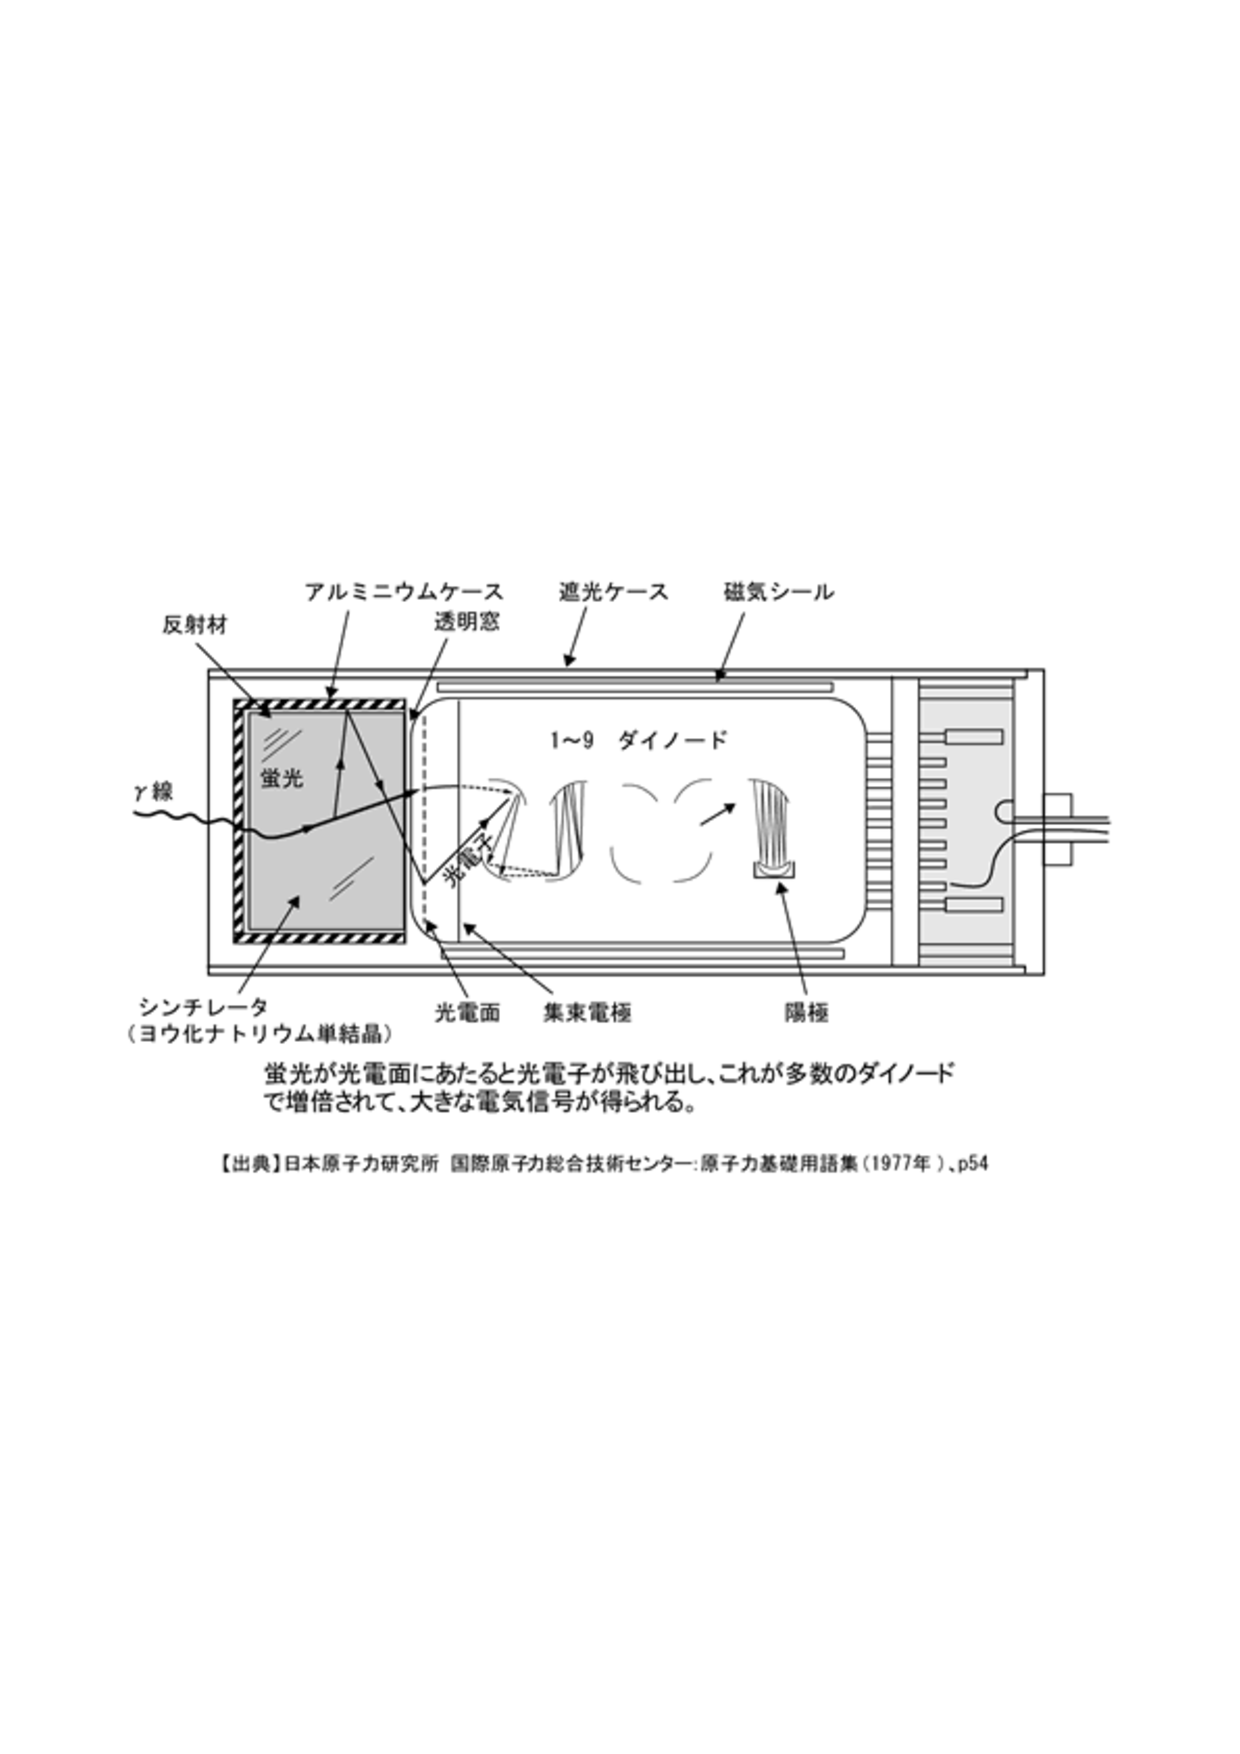
\includegraphics[bb=56 273 539 569,width=10cm]{scinti.pdf}
 \caption{シンチレータ検出器の仕組み}
 \label{031605_3Sep18}
\end{figure}

 より具体的にこの過程について調べよう.はじめにガンマ線とシンチレータ結晶が相互作用するのは,コンプトン効果,光電効果,電子対生成による.コンプトン効果はガンマ線と電子の弾性散乱であり,電子のエネルギーはその散乱角度$\theta$によって
\begin{align*}
 E=\frac{E_\gamma}{1+\frac{mc^2}{E_\gamma(1-\cos\theta)}}
\end{align*}
と表すことができる.この式からわかるようにコンプトン散乱は最大エネルギーを$2E_\gamma^2/(2E_\gamma +mc^2)$とする連続スペクトルを作るが,ガンマ線検出ではすぐ後に述べる光電効果,電子対生成の作る光電ピークと呼ばれるピークが大切であり,コンプトン散乱はあまり重要ではない.

光電効果はガンマ線が原子に入射すると電子が放出する現象のことである.これにより放出される電子のエネルギーは,仕事関数$W$として
\begin{align*}
 E=\hbar\omega -W
\end{align*}
で与えられる.電子が放出された原子は電子の再配列に伴って残りの$W$のエネルギーを放出し,結局全てのエネルギーが検出器に与えられることになる.このようにしてできるピークを光電ピークといい,入射ガンマ線の全エネルギーに対応していることからスペクトル解析では非常に大切なピークである.光電効果の断面積は原子の$Z^5$に比例するため,検出器の$Z$が大きければより多くの光電効果を起こすことになり,検出器として優れているということができる.

最後に電子対生成は,ガンマ線が電子と陽電子を作る反応のことであり,これは$\gamma$線のエネルギーが二つの粒子の静止エネルギーの和$1.022$MeV以上の時に発生する,つまり高エネルギーガンマ線の検出時に大切な反応である.生成した陽電子は原子内の他の電子と対消滅することで再び二本のガンマ線となる.この二本のガンマ線がいずれも検出器内で反応すれば,全エネルギーは$\gamma$線のエネルギーに等しく,光電ピークに一致する.しかしながら一本の$\gamma$線のみが反応すれば全エネルギーより$0.51$MeVだけ低いエネルギーになる.これをシングルエスケープピークという.二本とも検出器外へ逃げてしまえば全エネルギーより$1.02$MeVだけ低いエネルギーとなり,これをダブルエスケープピークという.

これら三つの相互作用の断面積の大きさを比較するため,例としてNaIの断面積の大きさを示したものが図\ref{032623_3Sep18}である.表からわかるように低エネルギーではコンプトン散乱が支配的であるが,高エネルギーでは光電効果と電子対生成が重要である.
 \begin{figure}[htb]
  \centering
  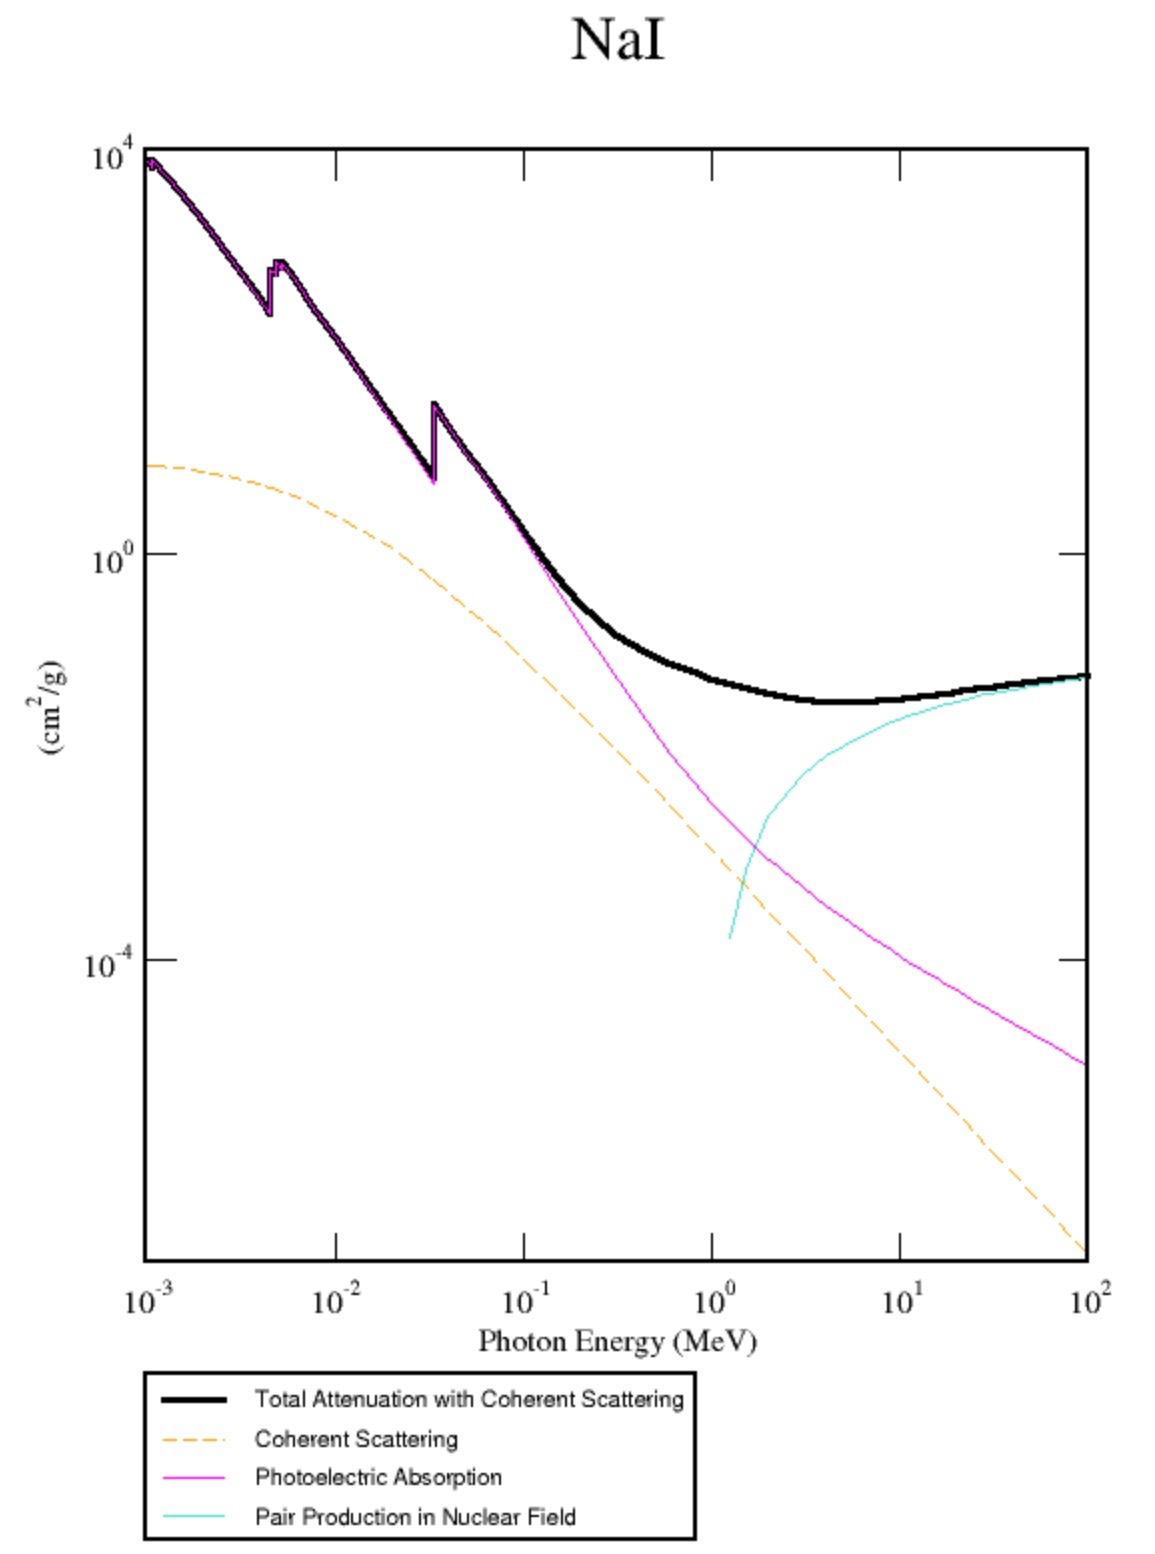
\includegraphics[bb=0 0 1155 1554,width=5cm]{NaI.jpg}
  \caption{NaIの反応断面積}
  \label{032623_3Sep18}
 \end{figure}



\subsection{GAGG}
 今回の実験で用いるのはセシウム添加Gd3Al2Ga3O12という結晶で通称GAGGと呼ばれる.GAGGは現在理化学研究所で$\gamma$線検出器として用いられているDALIと呼ばれるNaIシンチレータとPMTの組み合わせの後継候補として研究されている結晶で,その最大の利点は結晶のZが大きいので光電効果や電子対生成の反応断面積が大きく結果としてefficiencyが良いことである.したがってGAGGは時間の限られた実験や元々の反応断面積が非常に小さい実験に適した結晶であると言える.もう一つの利点はGAGGはNaIと違い潮解性がないことである.DALIはその潮解性により周囲を密閉する必要があり,多数のDALIを用いて立体角を稼ごうとした時に密閉分だけ不利である.
 \begin{figure}[htb]
  \centering
  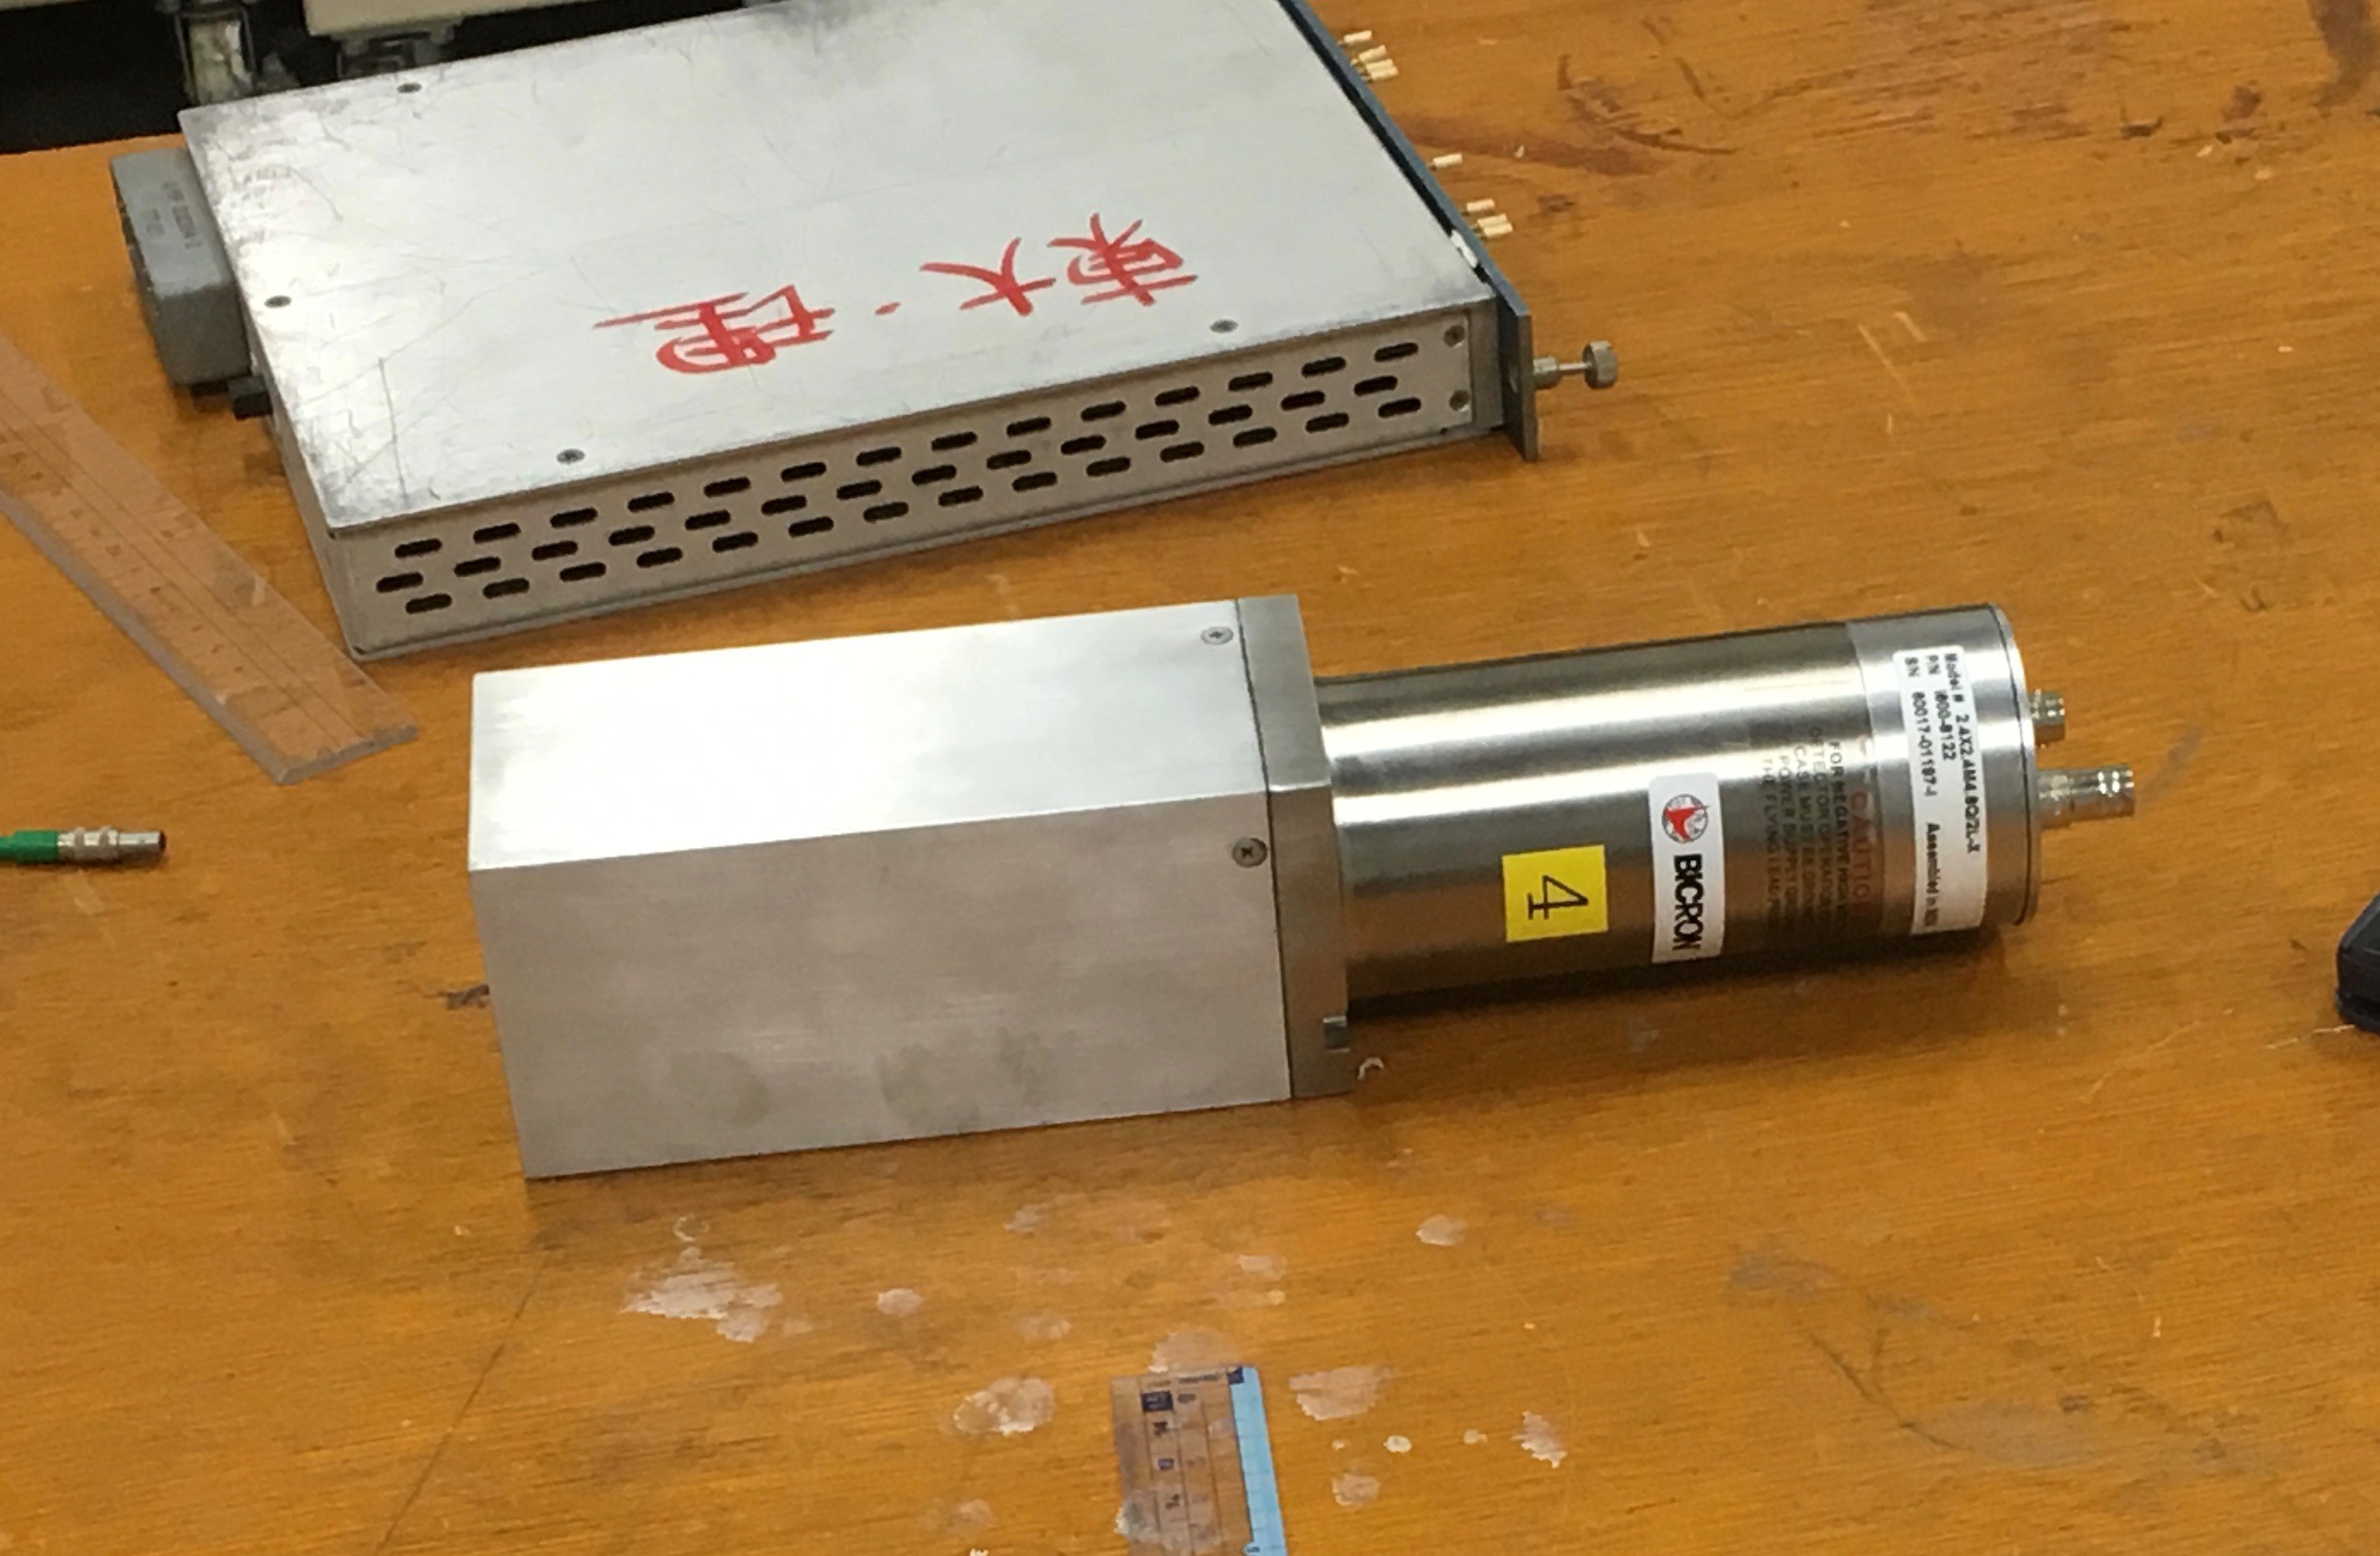
\includegraphics[bb=0 0 2467 1613,width=10cm]{DALI.jpg}
  \caption{DALI hongkong}
 \end{figure}


\subsection{実験の目的}
本実験の目的は,高エネルギーガンマ線に対するGAGGの応答を調べることである.Linearity,Resolution,Efficiency,Timing resolutionなどが主な解析対象である.特に今回の実験では新しく世界最大級の$10\times 3.5\times 3.5\mathrm{[cm^3]}$のGAGGを用意しており,このGAGGの特性について詳しく調べることを意図している.
  \begin{figure}[htb]
   \centering
  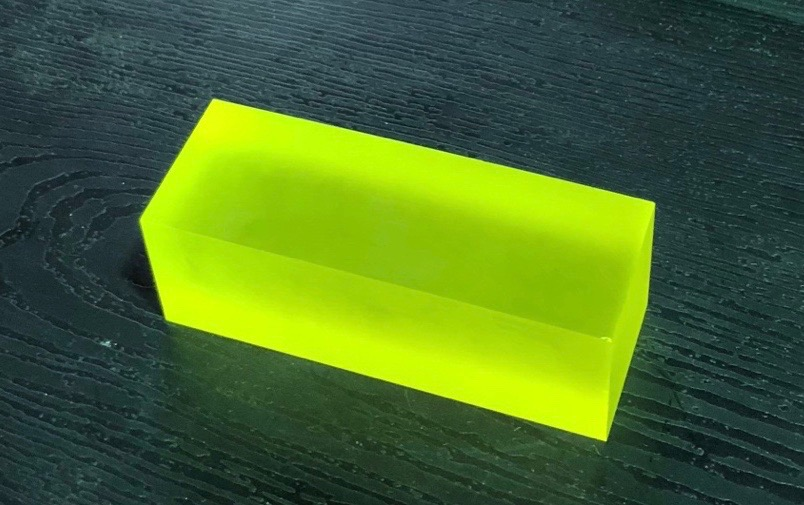
\includegraphics[bb=0 0 804 505,width=10cm]{GAGG.jpg}
  \caption{世界最大級のGAGG結晶}
  \label{005006_3Sep18}
  \end{figure}




\section{予備実験とその結果}
まずは本郷の319号室で行われた予備実験について,はじめの数章で実験全体を通して用いられたセットアップについてのべる.その後GAGGの性能をテストする複数の実験についてまとめる.

\subsection{結晶とPMT}
予備実験で用いた結晶とPMTについて解説する.結晶としては本実験用に用意された$10\times 3.5 \times 3.5 \mathrm{[cm^3]}$のGAGG結晶を用いた.


PMTは三種類用いた.これら三種類のPMTはそのまま本実験でも用いられたものであるが,このうち一つは円柱型,残りの二つは立方体型で形が異なっておりPMTと結晶の結合に当たっては別々の方法を取る必要があった.
\begin{table}[htb]
 \centering
 \begin{tabular}{|c|c|c|}
  PMT型番&形状 &極性 \\
  & & \\
  & & \\
  & & \\
 \end{tabular}
\end{table}
GAGGの蛍光波長は$520$nmとNaIの$420$nmに比較して長めであり,GREEN EXTENDED PMTはこの長波長に適したPMTである.その様子を示したのが図\ref{032823_3Sep18}で,GREEN EXTENDEDはより長波長側にピークを持っていることがわかる.
\begin{figure}[htb]
 \centering
 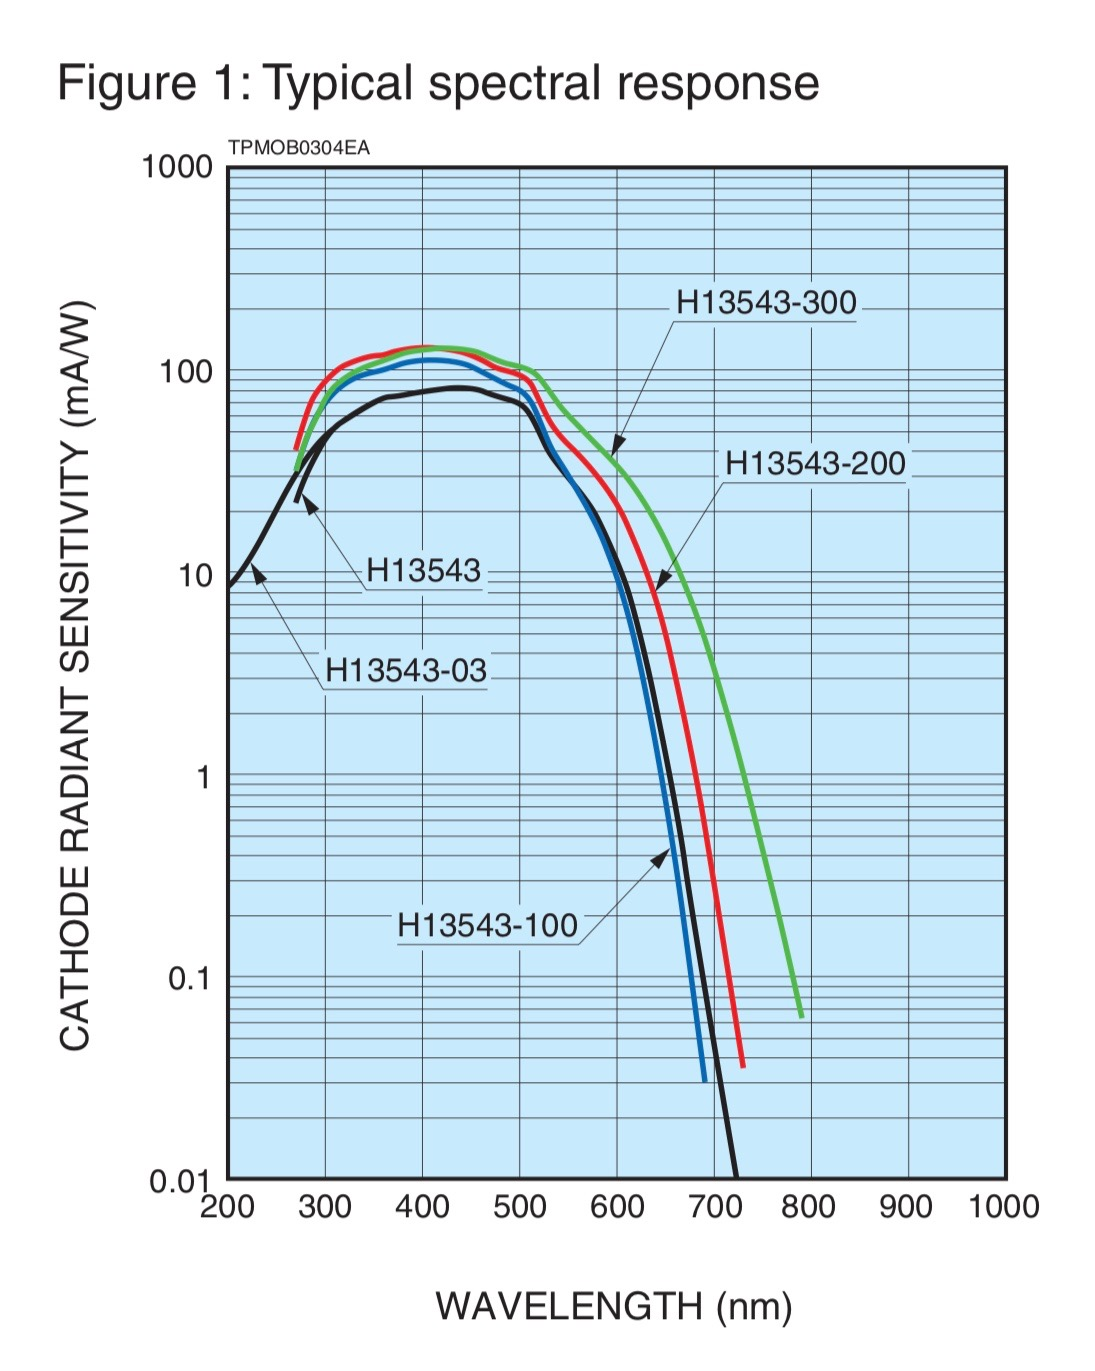
\includegraphics[bb=0 0 1095 1371,width=5cm]{PMTgreen.jpg}
 \caption{各種PMTの波長依存性}
 \label{032823_3Sep18}
\end{figure}



結晶は反射材としてテフロンテープまたはESRによって巻かれる.その様子は図\ref{023945_3Sep18}に示されている.
\begin{figure}[htb]
 \centering
 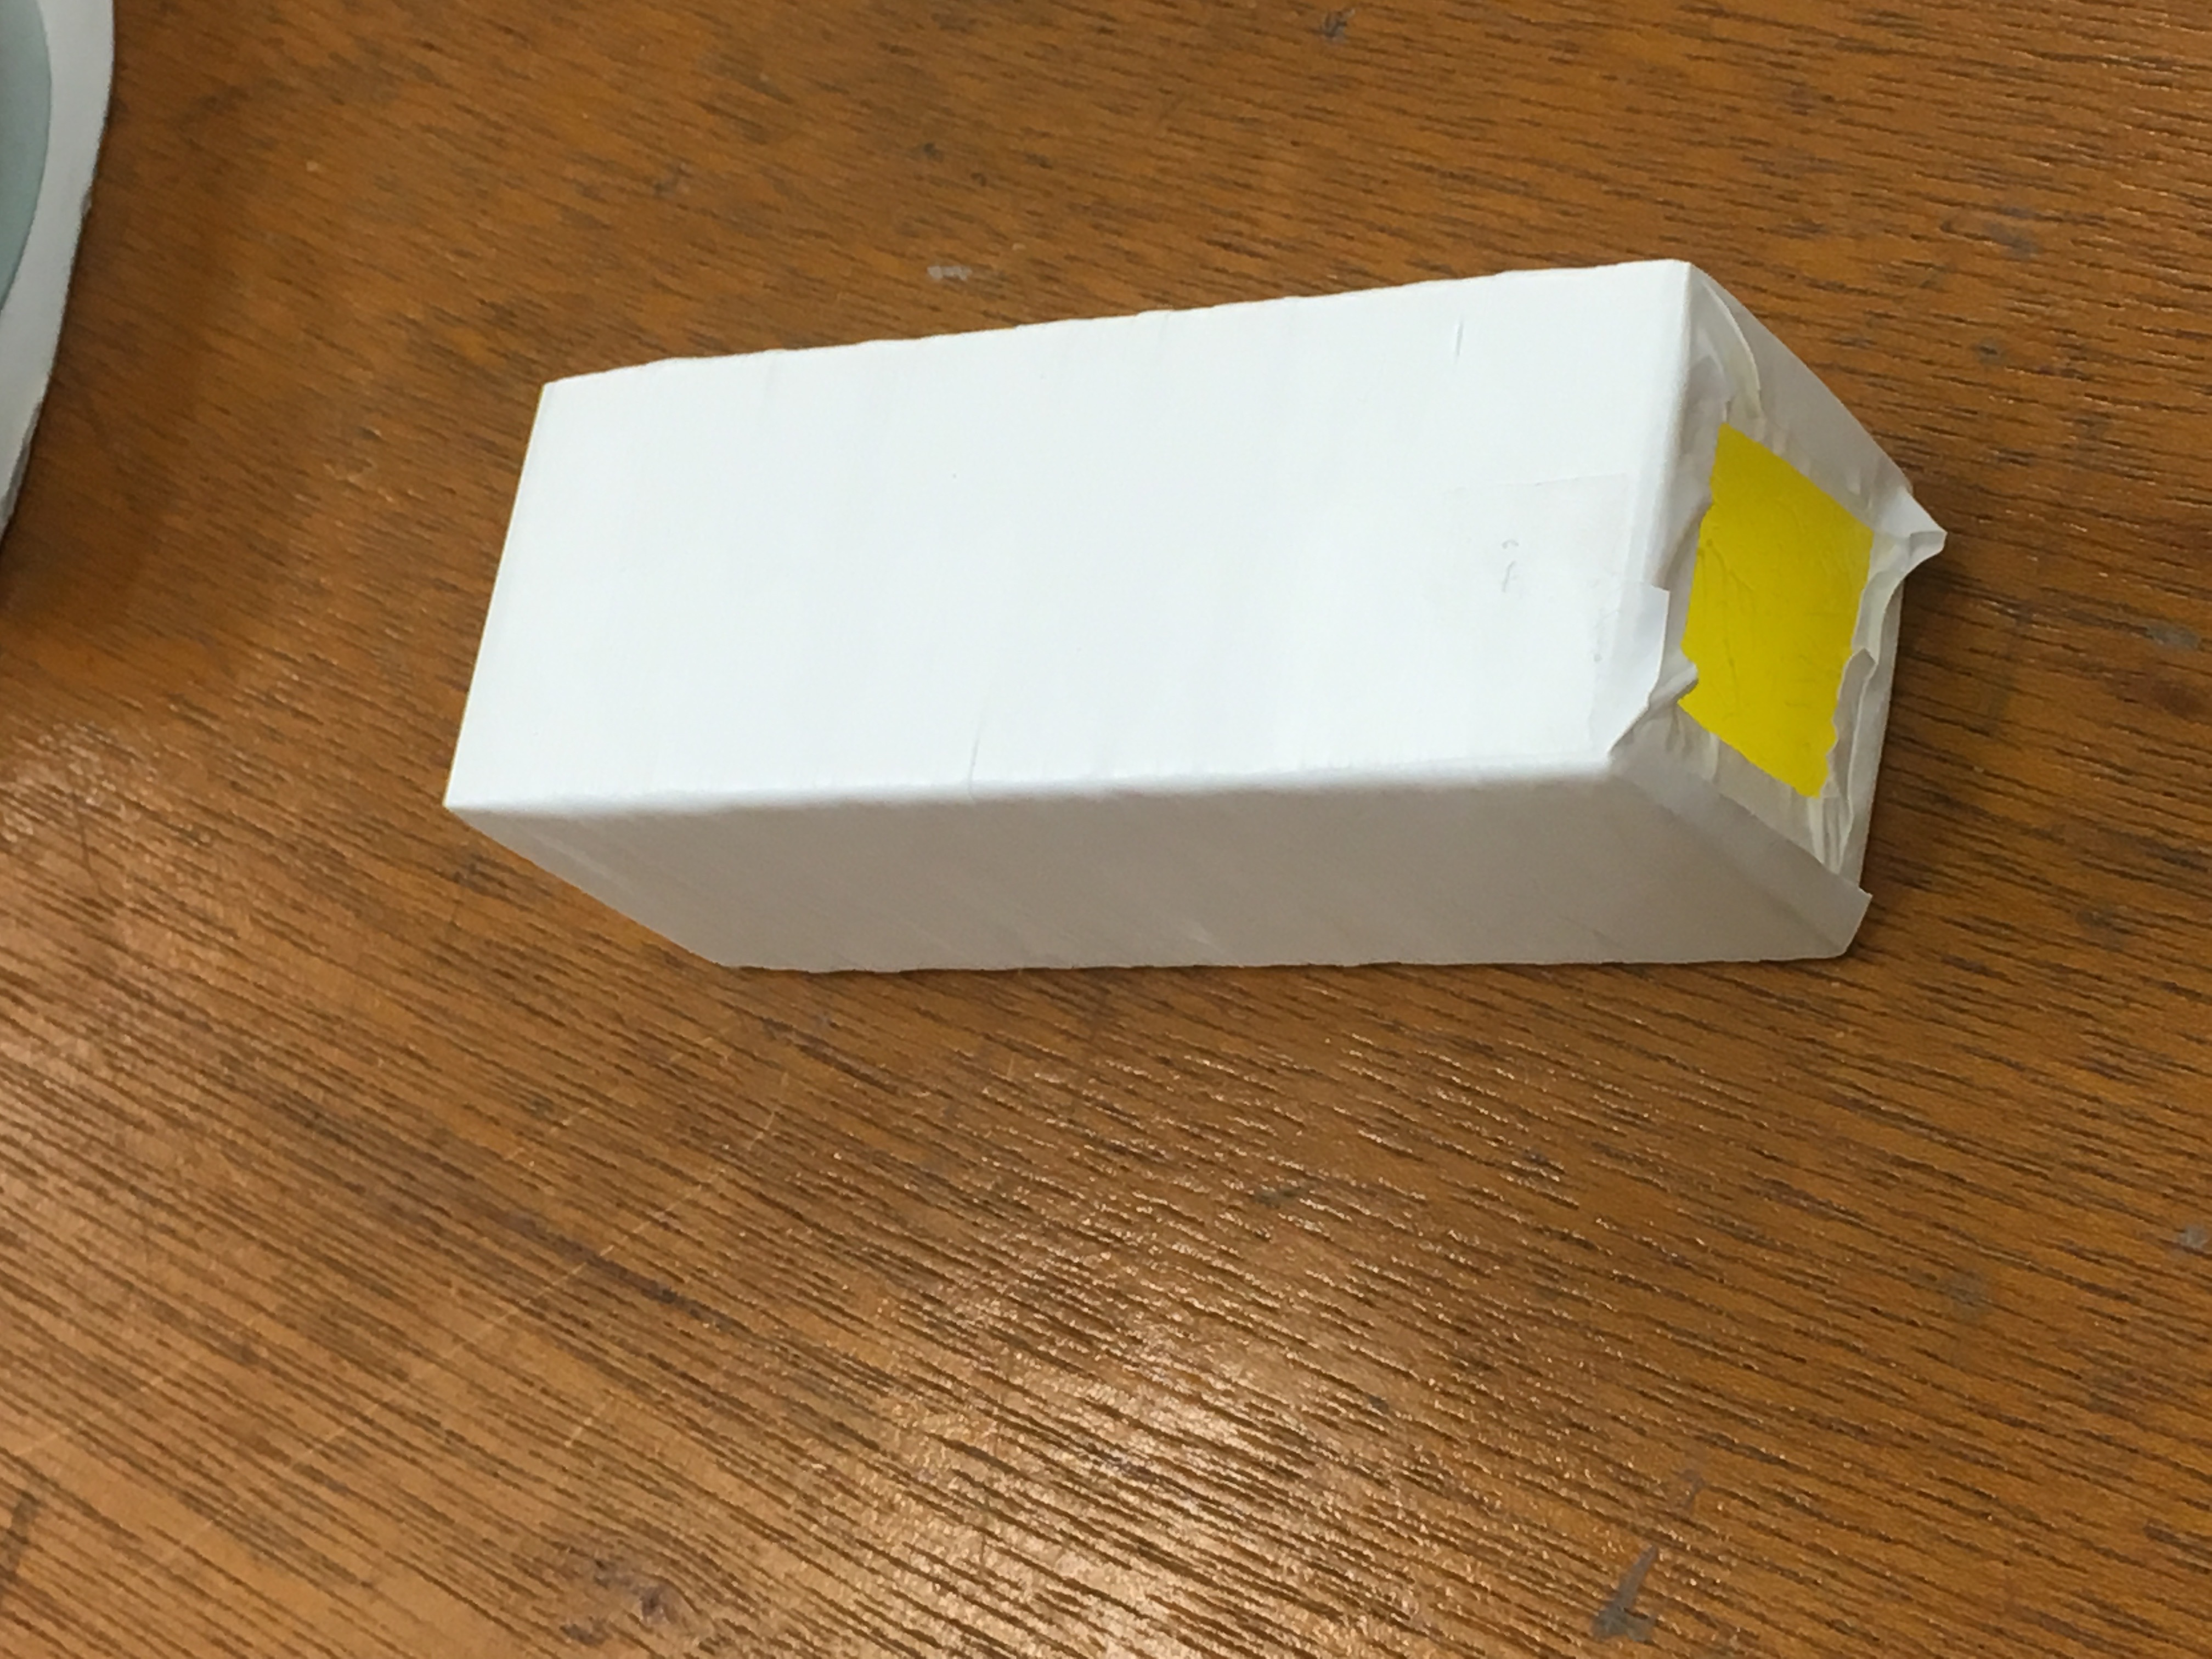
\includegraphics[bb=0 0 4032 3024,width=10cm]{tefron.jpg}
 \caption{反射材としてテフロンを巻かれたGAGG}
 \label{023945_3Sep18}
\end{figure}

PMTと結晶の結合は(グリース)によって行われた.グリースは光をよく透過させるため,なるべくPMTおよび結晶と近い屈折率をもつ方が良い.PMTと結晶の結合は実験中もっともバラツキの出る要素の一つであり,この工程をいかに完璧に実行するかというのが大切である.さらにグリースによって結合されたPMTと結晶は,遮光テープを巻いたアクリルケースに入れられることで遮光された.この様子は図\ref{033232_3Sep18}に示されている.
\begin{figure}[htb]
 \centering
 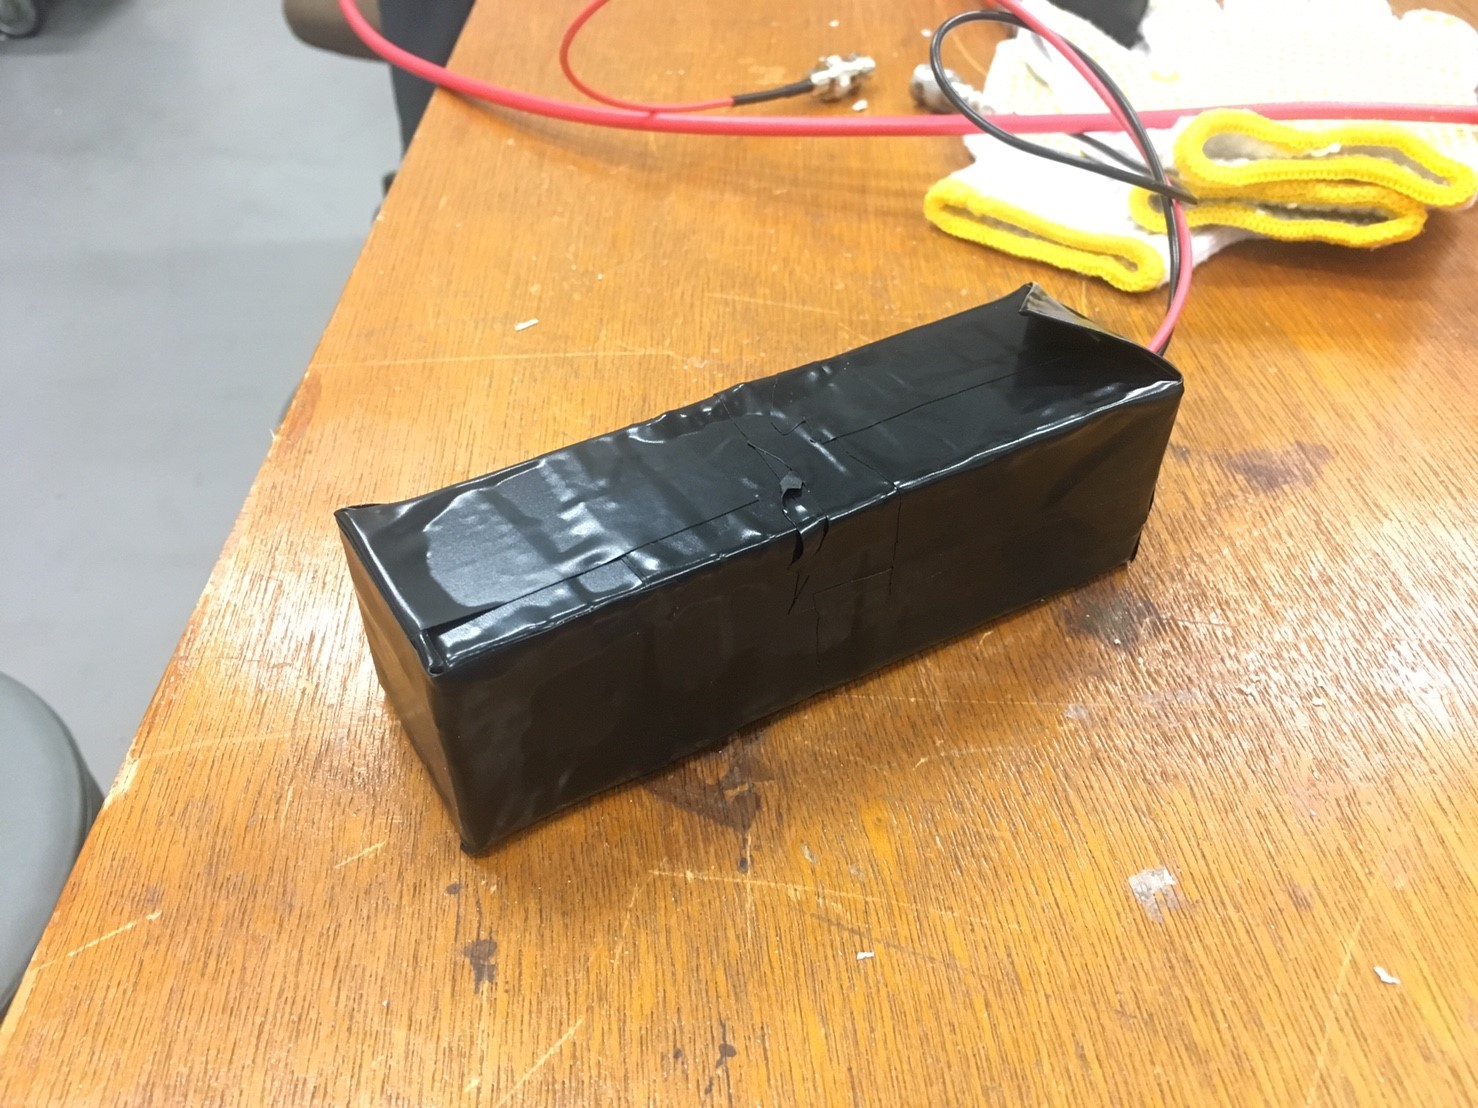
\includegraphics[bb=0 0 1478 1108,width=10cm]{akuriru.jpg}
 \caption{アクリルケースに収められたGAGG結晶}
 \label{033232_3Sep18}
\end{figure}
本実験ではより本格的なPMTケースが用意され,このケースは利用されなかった.



\subsection{DAQのセットアップ}
本郷での実験で用いられたDAQはQDCと呼ばれる手法で,信号を

実験は図\ref{012905_3Sep18}のようなセットアップで行われた.用いられたモジュールは表にまとめられている.
\begin{figure}[htb]
 \centering
 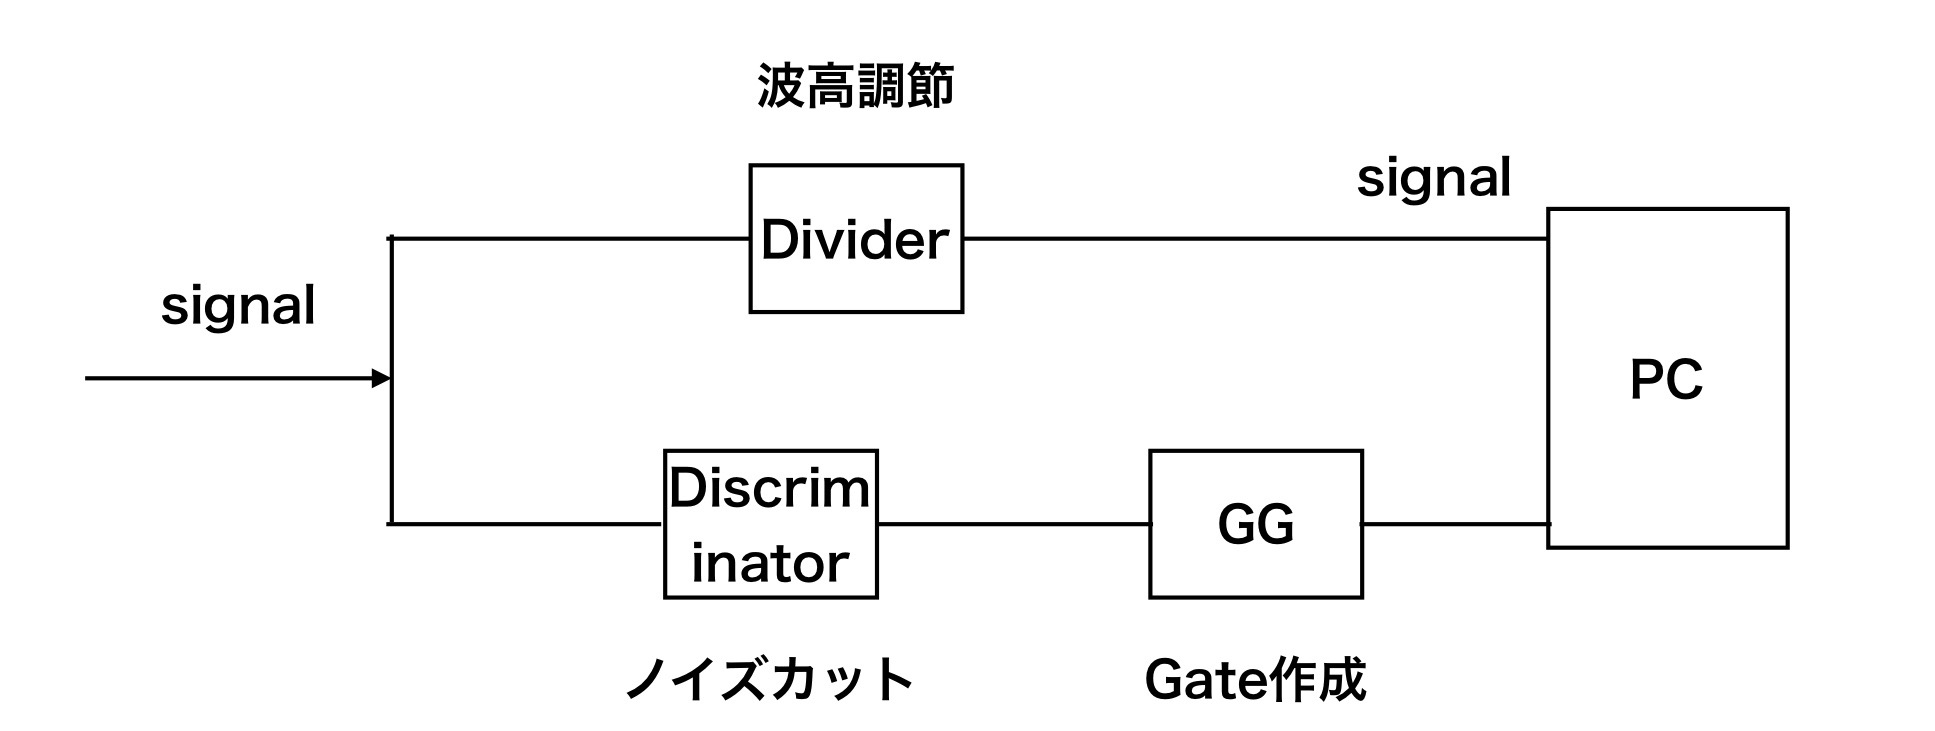
\includegraphics[bb=0 0 1935 731,width=10cm]{QDC.jpg}
 \caption{QDC回路}
 \label{012905_3Sep18}
\end{figure}



\begin{table}[htb]
 \centering
 \begin{tabular}{|c|c|c|}
  モジュール&型番 & \\
  高電圧供給& & \\
  Discriminator& & \\
  QDC& & \\
 \end{tabular}
\end{table}

この回路はPMTの出力信号とその出力信号をトリガーとするGateからなっており,Gate信号ではノイズ信号でGateを開かないようにあらかじめDiscriminatorでノイズをカットしている.
 実験を通して変えられるパラメータは,PMTにかける電圧,ノイズ信号を除去するためのスレッショルド値,積分時間を指定する,および信号の遅らせ具合を指定するDelay timeである.このうちスレッショルド値は余程エネルギーの低いガンマ線を測ろうとしない限りほとんど測定結果に影響しない(本実験では,NaIの$0.511$MeVのピークがノイズに埋もれてしまうケースが稀に発生した.).また,Delay timeも本質的ではないので,実質的には電圧と積分時間のみが重要である.積分時間は長くとればそれだけ信号の減衰を結果に反映させることができるが,同時にノイズの増加や次の信号が来た時にそれを測定できないなどの問題が生じる.電圧については後述するように,PMTによって適正な電圧が存在し,その電圧に設定することが実験を成功させるために必要である.





\subsection{線源と検出器}
γ線源としては以下の表2に示すものを用いた.
  \begin{table}[htb]
  \centering
\begin{tabular}{|c|c|c|}
 線源名& & \\ \hline
 Cs& & \\
 Co& & \\
 Na& & \\
\end{tabular}
   \caption{実験で用いた線源一覧}
  \end{table}

線源は検出器から一定の長さのところに設置される.これは特筆することがなければ本実験では$10$cmとして実験を行った.


\subsection{GAGG結晶からの信号}
まずはGAGGとPMTの組み合わせで得られる生信号をいくつか
(これは厳しいかもな,,,)



\subsection{電圧の依存性}
色々なPMTとの組み合わせで電圧の値を変え,Resolutionを測定する実験を行った.実験を通して




\subsection{実験についてのいくつかの指摘と考察}
予備実験を行っている間に気が付いたことについていくつか箇条書き形式で指摘しておく.
\begin{itemize}
 \item 小型のPMTを用いる場合GAGG結晶の方がPMTよりも大きいため,GAGGとPMTの接続面の光漏れをどう阻止するかが重要である.今回は反射材を貼り付けることで対処したが,この反射材がグリースで乱れてしまうことが多く,対策を講じるべきである.
 \item PMTは電圧をかけ始めてから安定した動作を見せるまでに$30$分程度かかり,電圧をかけ始めてすぐに測定をすると望ましい結果が得られないことがある.しかし今回の理化学研究所で行われた実験では,PMTとGAGGの組み合わせを変えて実験する必要があったため(後述)あまり良くないとわかっていながらも電圧をかけてすぐ測定を行った.
 \item GAGGはDALIに比較して非常に信号の波高が高く,今回用いたQCDで測るためには波高を小さくする必要があった.これはより高いエネルギーを測る本実験でより顕著であり,波高を小さくするために用いたDividerは(Attenuatorに比べれば大分ましなものの)Resolutionの悪化に貢献していると考えられる.
\end{itemize}







\newpage
\section{10MeVのγ線の検出実験}

\subsection{実験の基本設計}
本実験のメインテーマである高エネルギーのガンマ線検出にあたり,まずは高エネルギーのガンマ線を人為的に作る必要がある.そこでAl(p,$\gamma$)Siの$992$keVの反応を用いた.これはアルミニウムに高エネルギーのプロトンビームを入射するとSiの励起状態が出来,そこからよりエネルギーの低い状態になる時にSiからガンマ線が放出される過程であり,そのエネルギーについては下の図\ref{035121_3Sep18}にまとめられているが,この左端にある反応が$11$MeVの$\gamma$線を放出する反応で,今回の実験で主要に観測されるものである.
\begin{figure}[htb]
 \centering
 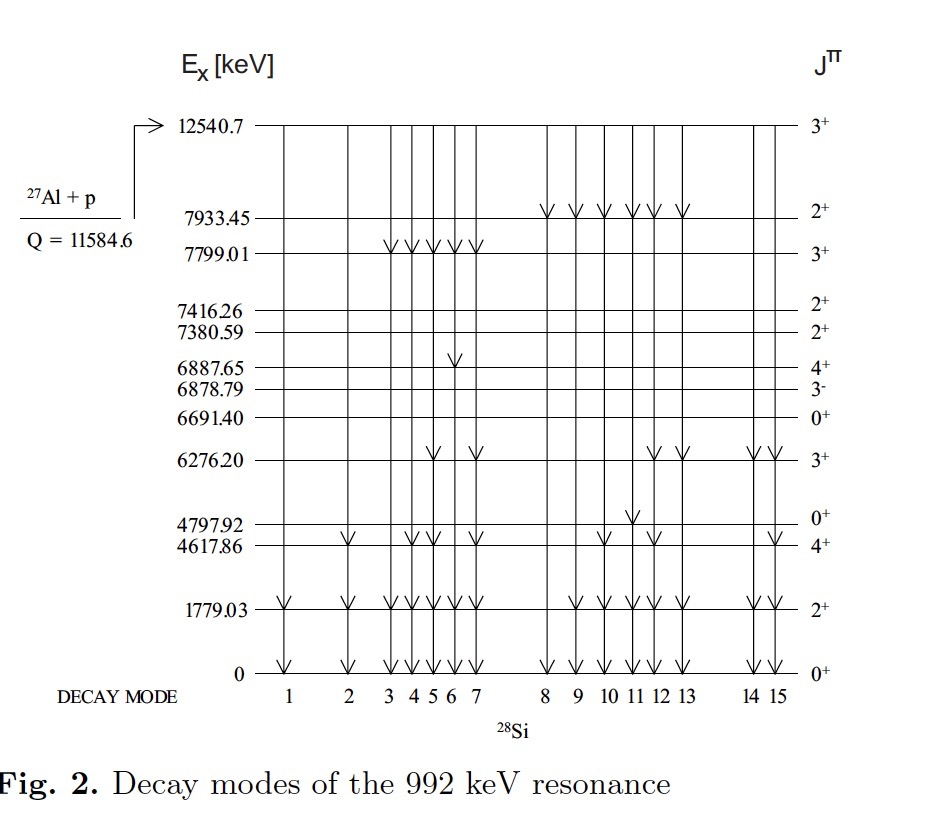
\includegraphics[bb=0 0 936 825,width=8cm]{energy.jpg}
 \caption{$992$keVの遷移の様子}
 \label{035121_3Sep18}
\end{figure}


この反応は今までによく研究がなされており,Ge検出器で測ったスペクトルは図\ref{025209_3Sep18}のようになる.
\begin{figure}[htb]
 \centering
 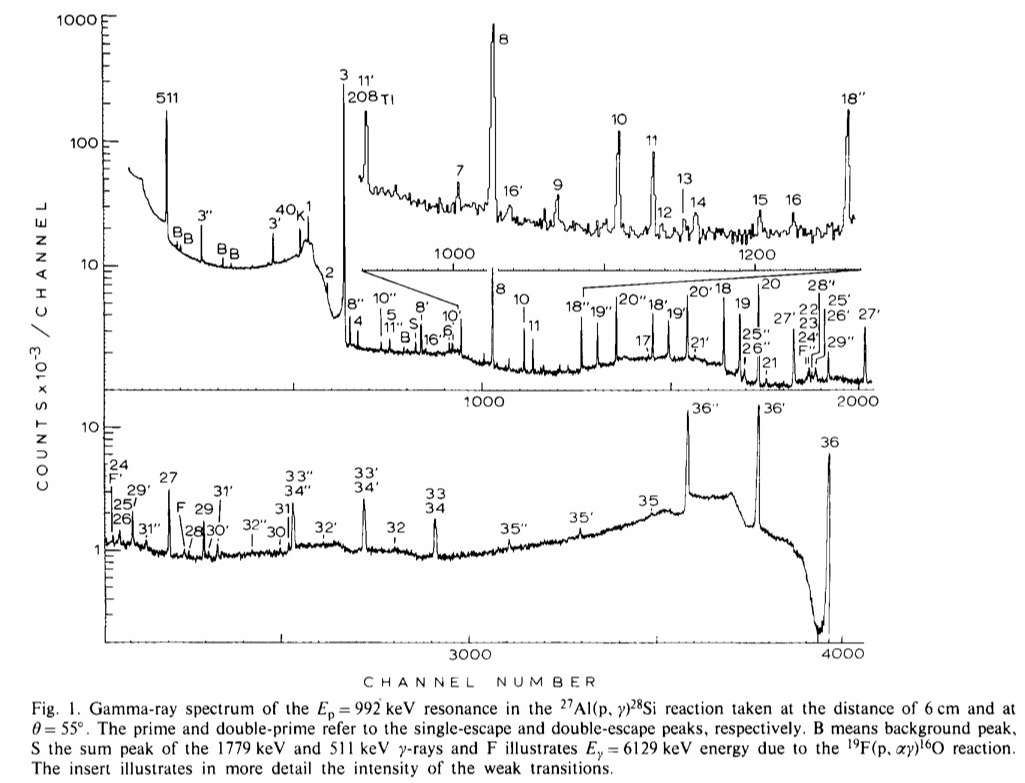
\includegraphics[bb=0 0 1025 783,width=8cm]{spectrumGe.jpg}
 \caption{Ge検出器で得られたスペクトル}
 \label{025209_3Sep18}
\end{figure}
従ってGAGG検出器で得られたスペクトルとこれらのスペクトルを比較することにより,各スペクトルを同定することが期待される.




\subsection{加速器について}
今回の実験では理化学研究所ペレトロン室にある静電加速器が用いられた.この加速器は$3$MeVまで粒子を加速することができ本実験に適している.また加速器の仕組みは図\ref{035816_3Sep18}に示されている.イオン源から放出された負イオンはまず一段階目の静電場で加速された後,荷電ストリッパーガスとの衝突によって電子を奪われ正に帯電され,さらに二段階目の静電場で加速される.このようにすることで一段階で加速するよりも低い電場で加速することができ効率的である.本実験では$992$keVの共鳴を用いるため,$1$MeVのプロトンビームを用いられた.
\begin{figure}[htb]
 \centering
 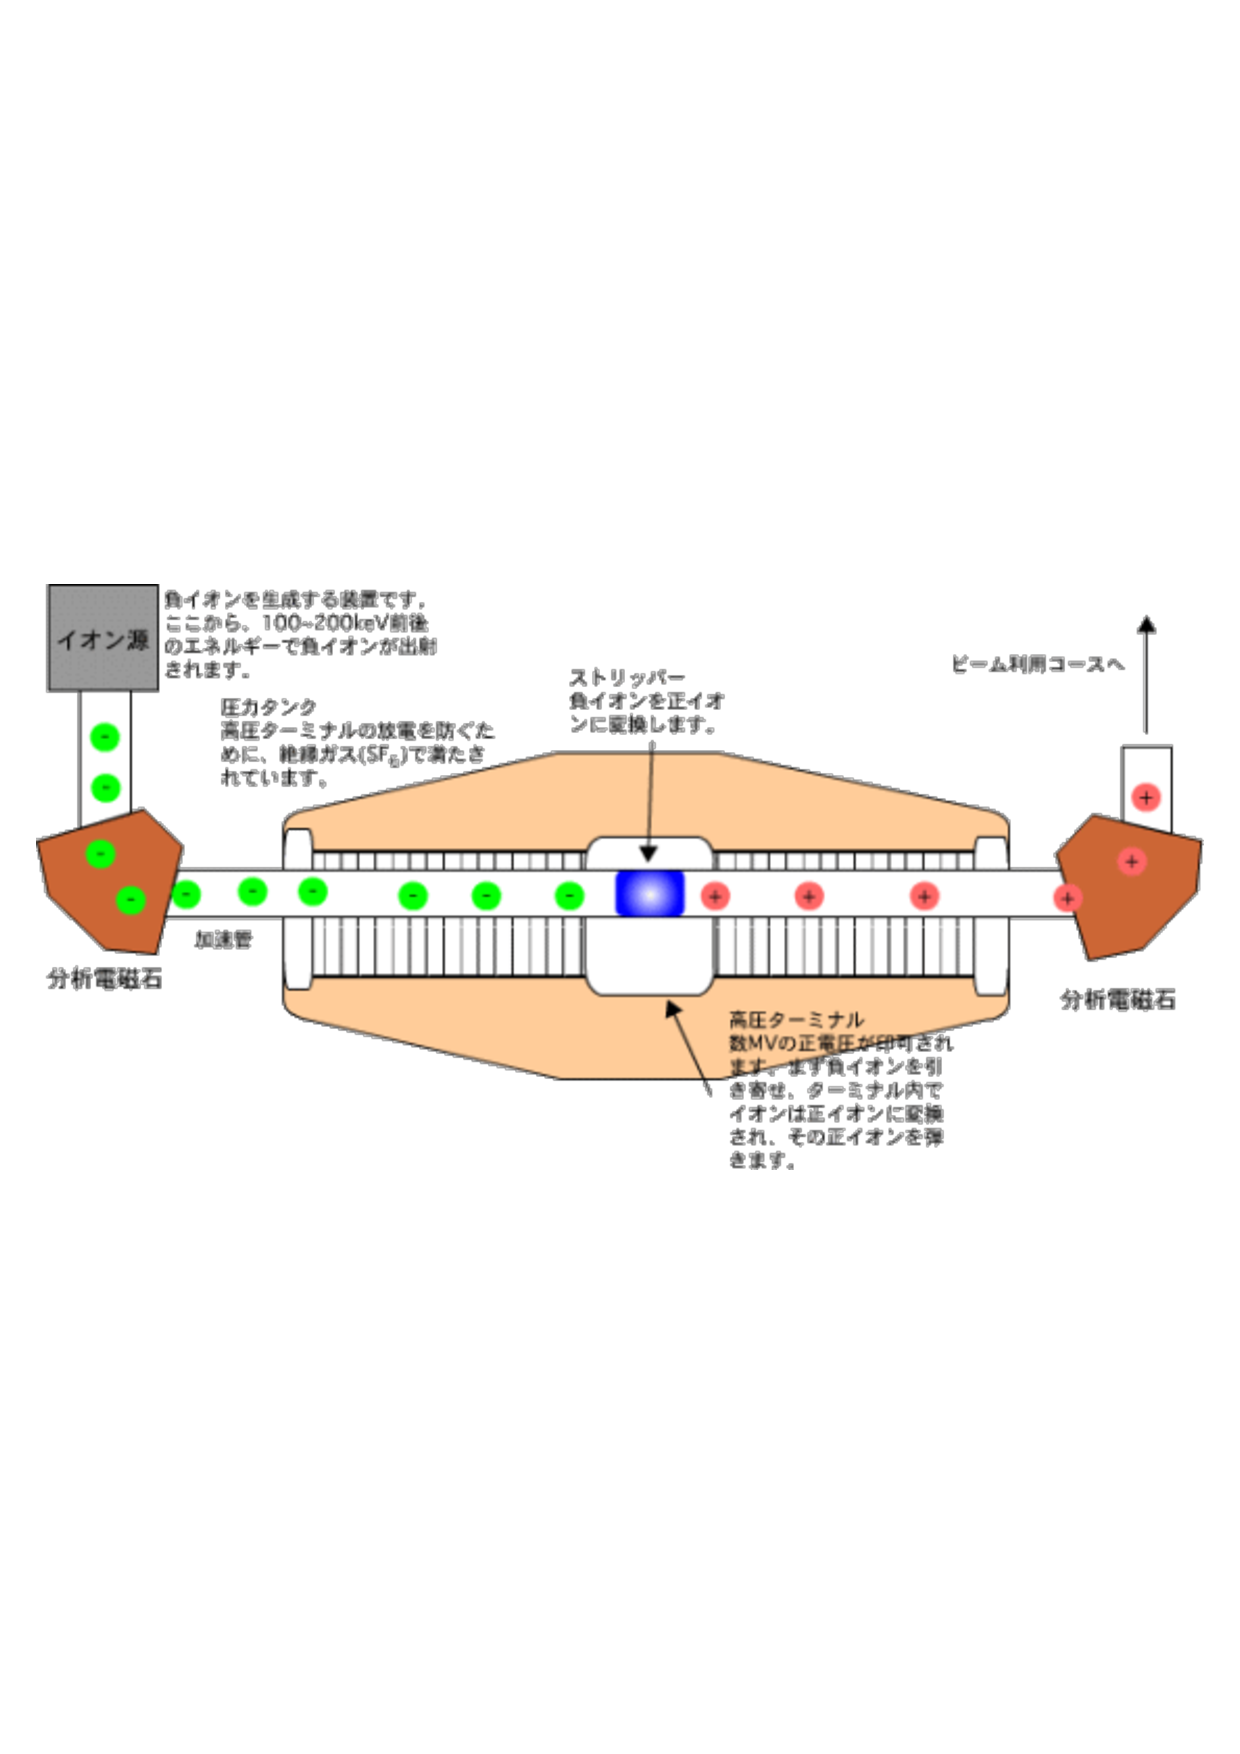
\includegraphics[bb=17 280 578 562,width=10cm]{tandem.pdf}
 \caption{ペレトロン加速器の原理}
 \label{035816_3Sep18}
\end{figure}


\subsection{ターゲットおよび検出器の配置}
 ターゲットはプラスチックでできたターゲットホルダーに固定されたmmのアルミニウム箔であり,この厚さのターゲットはベーテブロッホの公式
\begin{align*}
 -\frac{1}{\rho}\frac{dE}{dx}=D\frac{Z}{A}\frac{z^2}{\beta^2}\left(\log\left[\frac{2mc^2\beta^2}{I(1-\beta^2)}\right]-\beta^2\right)
\end{align*}
に従って,$1$MeVのプロトンビームのエネルギーを
\begin{align*}
 a
\end{align*}
だけ減少させると期待される.アルミニウム泊に繋がれた導線からプロトンビームの電流を測ることができるようになっている.このターゲットホルダーがビームライン上の真空管に設置される.


今回用いた検出器はDALI hongkongが9台,GAGG結晶が4つ,PMTが4つであり,DALIは常に同じ配置で固定され,GAGGはいくつかのPMTとの組み合わせで測定された.$4$つのGAGGおよび$4$つのPMTについては表にまとめられている.

これら検出器はビームラインを取り巻くように図のように設置された.予備実験と同じく,検出器とターゲットの距離がおよそ$10$cmになるように設置されている.
\begin{figure}[htb]
 \centering
 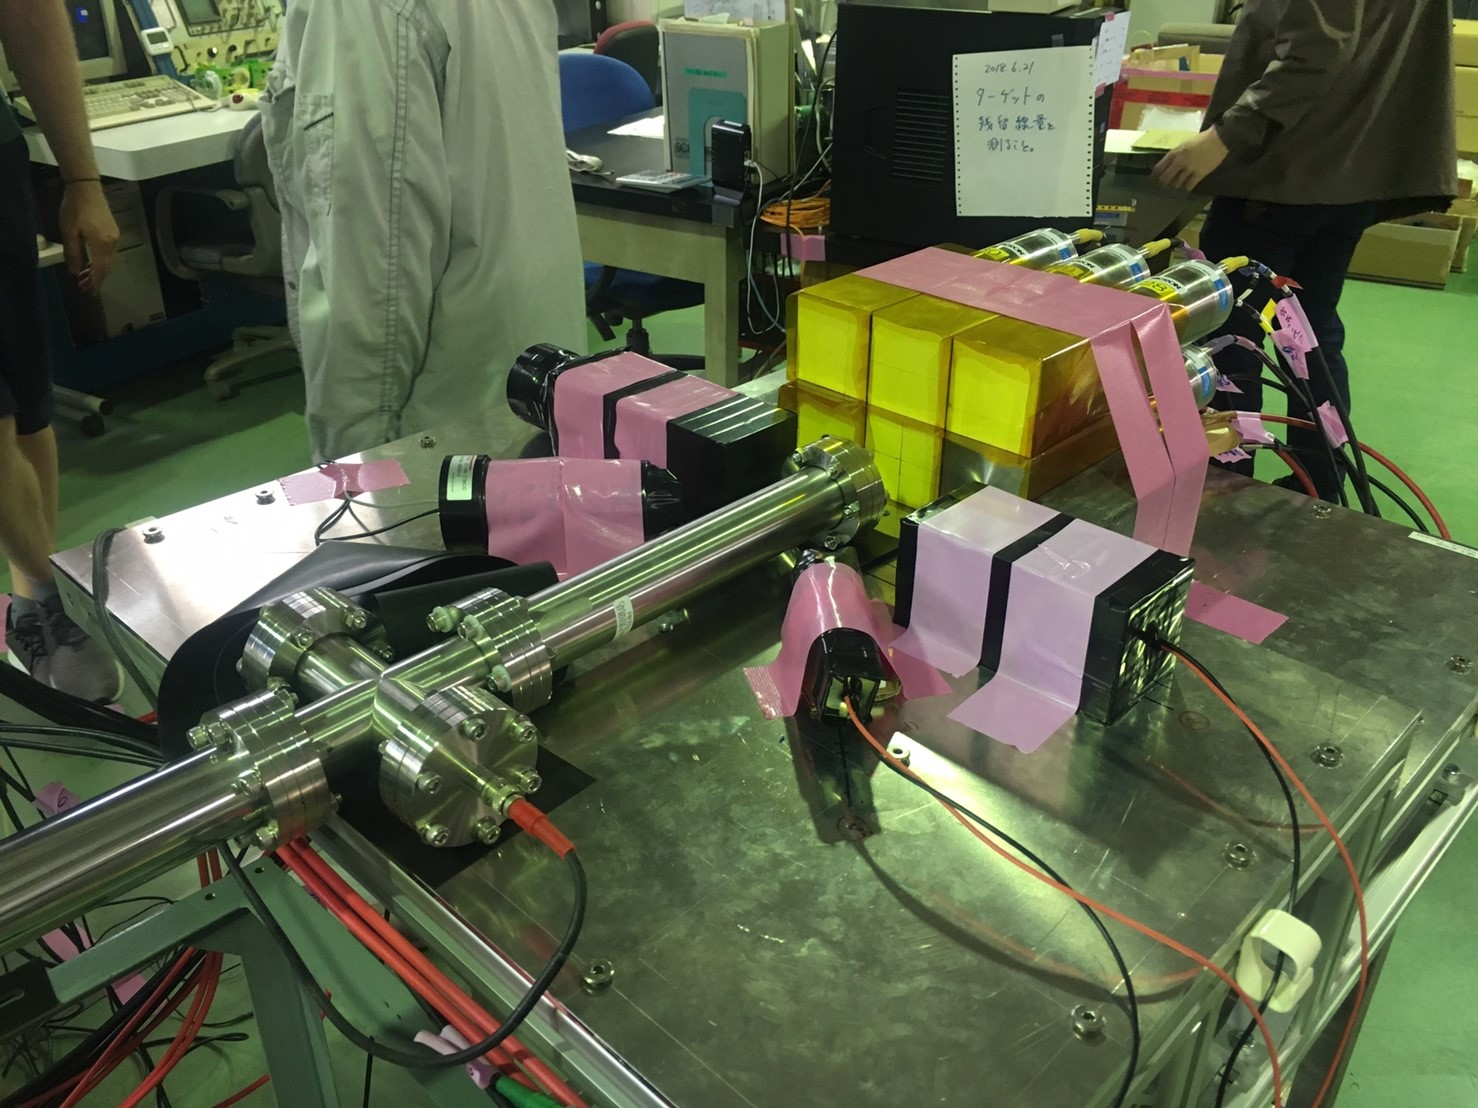
\includegraphics[bb=0 0 1478 1108,width=10cm]{align.jpg}
 \caption{検出器の配置の様子}
\end{figure}
 







\subsection{データ取得のセットアップ}
 本実験でのDAQには二種類の回路が用いられた.まず一つは予備実験でも用いられたQCDであり,予備実験で用いた図を複数チャンネル用に拡張したものでその様子は図\ref{041815_3Sep18}に示されている.これはGAGGの測定に用いられた.
\begin{figure}[htb]
 \centering
 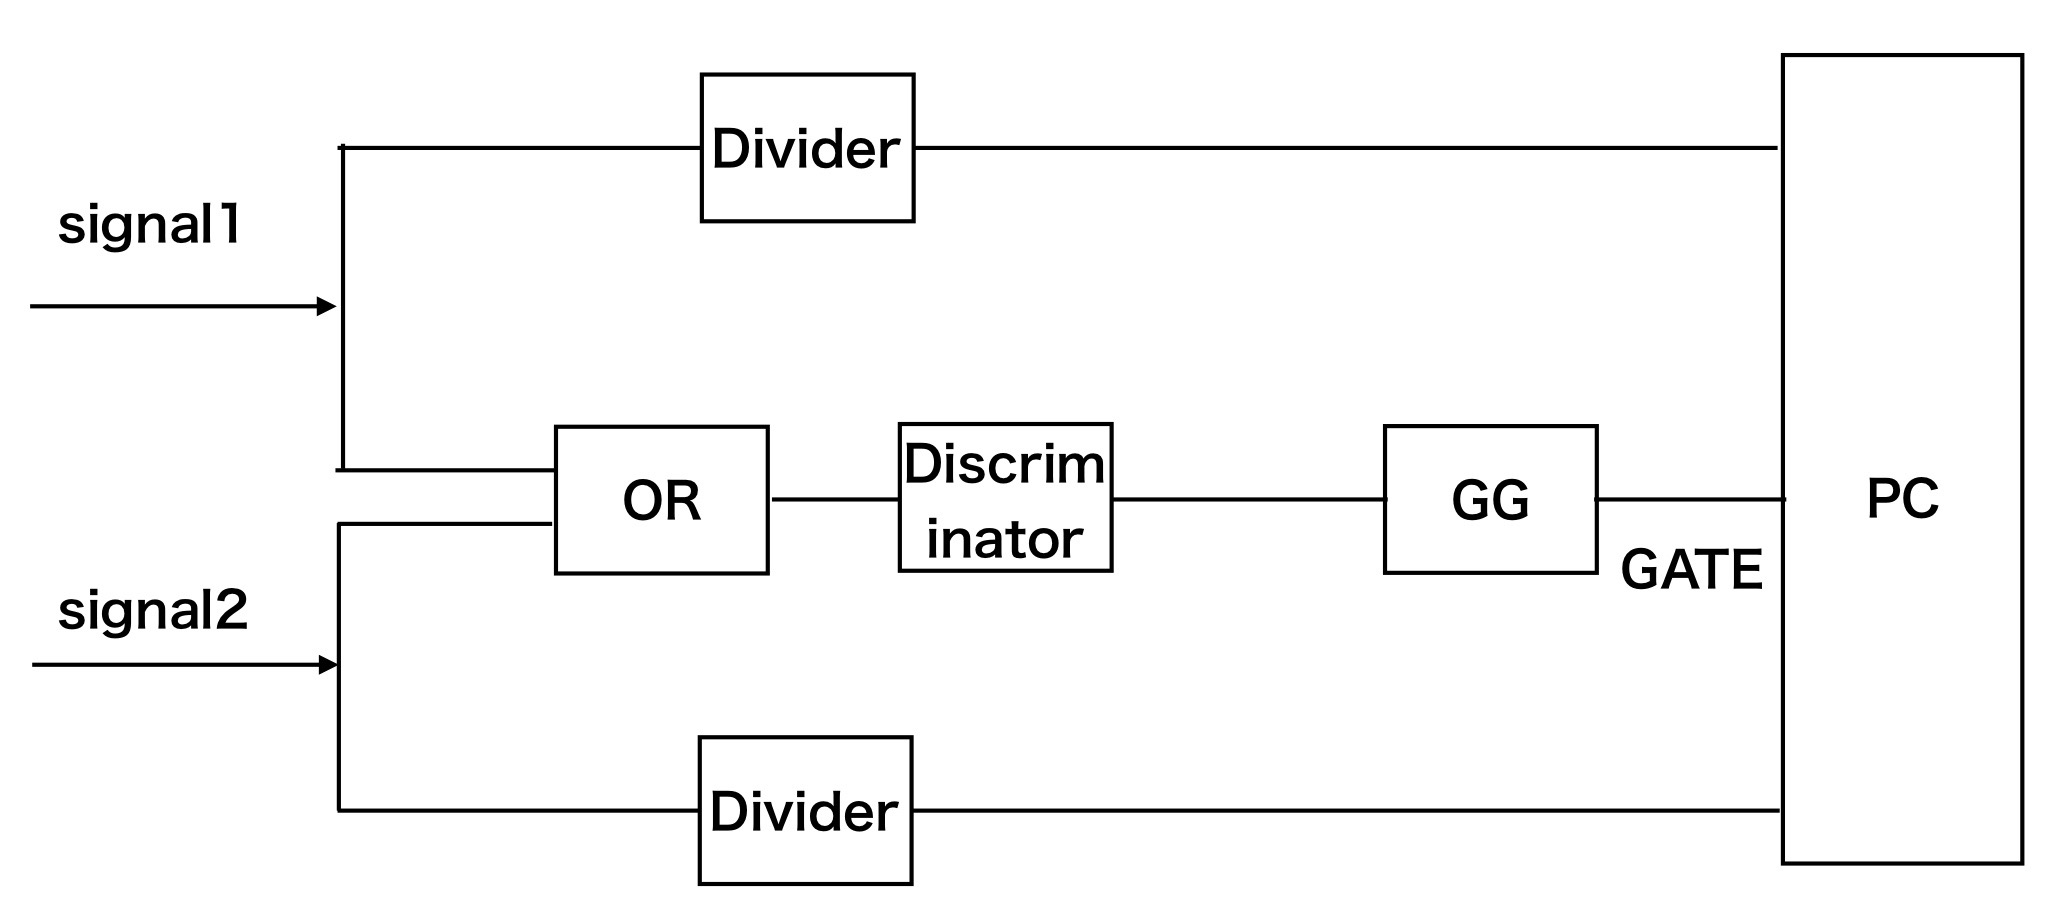
\includegraphics[bb=0 0 2069 911,width=10cm]{QDC2.jpg}
 \caption{QDC回路}
 \label{041815_3Sep18}
\end{figure}

もう一つはADCと呼ばれるもので,これはQDCと異なり自動で信号を積分することができる.回路の概要は下図に示されており,使われたモジュールは表にまとめられている.





この回路には


\subsection{実験のタイムライン}
 本実験は二日間に渡って行われた.実験は以下の表\ref{044628_3Sep18}および表\ref{045055_3Sep18}の通り実行されデータが取られた.ただしA,B,C,Dは前述の$4$つのGAGG結晶を,normalなどはPMTを表す.

\begin{table}[htb]
 \centering
 \begin{tabular}{|c|c|c|c|c|c|}\hline
  回数&A      &B        &C      &D        &プリアンプの有無 \\\hline
     1&normal &RT       &GN     &Bialcali &なし\\\hline
     2&GN     &Bialcali &normal &RT       &なし\\\hline
     3&RN     &Bialcali &なし   &normal   &なし\\\hline
     4&RN     &Bialcali &なし   &normal   &Aのみあり\\\hline
     5&RN     &Bialcali &なし   &normal   &Aのみあり\\\hline
 \end{tabular}
 \caption{ADCによる測定}
 \label{044628_3Sep18}

 \begin{tabular}{|c|c|c|}\hline
 回数&A      &D      \\\hline
 1&normal &RN     \\\hline
    2&RN     &normal \\\hline
\end{tabular}
 \caption{QDCによる測定}
 \label{045055_3Sep18}
\end{table}




\subsection{実験データ}


\subsection{解析}


\subsection{今後の展望}





\end{document}